\documentclass[11pt]{scrartcl}

% standard packages
\usepackage[utf8]{inputenc}  % input in UTF-8
\usepackage[T1]{fontenc}  % output in T1 fonts (westeuropaeische Codierung)
\usepackage{lmodern}  % latin modern fonts
\usepackage[ngerman]{babel}  % deutsches Sprachpaket, neue Rechtschreibung

% Seitensetup
\usepackage{scrlayer-scrpage}  % Seitenformatierung durch KOMA-interne Optionen
\usepackage[top=4cm, bottom=4cm]{geometry}  % Seitengeometrie (kann durch KOMA ersetzt werden, hab ich aber nicht geschafft)
\usepackage[hypcap=false]{caption, subcaption}  % caption editing - hypcap warning with hyperref
\usepackage{array}  % table editing

% additional packages
\usepackage{amsmath, amssymb, amstext}  % math packages (American Math Society)
\usepackage{bm}
\usepackage{icomma}  % Kommata in Dezimalzahlen verursachen keinen Abstand mehr
\usepackage{graphicx}  % Bilder einfügen
\usepackage{float} %Bilder placement
\usepackage{pdfpages}  % PDF als vollständige Seiten einfügen
\usepackage{lastpage}  % referenziert die letzte Seite
\usepackage[separate-uncertainty=true]{siunitx}  % bessere Darstellung von Einheiten
\usepackage{makecell} %Dicke Tabellenstriche
%\usepackage{datatool}
\usepackage[hidelinks]{hyperref}  % hyperref verlinkt Referenzen - hidelinks entfernt borders um links

% package setups
% Kopf- und Fußzeile durch KOMA
\pagestyle{scrheadings}  % KOMA darf entscheiden
\clearpairofpagestyles  % reset
\setkomafont{pageheadfoot}{\normalfont}  % Standardschrift in Kopf- und Fußzeile
\captionsetup{format=plain, font=small, labelfont=bf} %Better caption, Abbildung ist FETT
%\setlength{\headheight}{27.2pt}  % benötigte Höhe Kopfzeile (warning von scrlayer-scrpage, wird aber automatisch so gerendert, falls diese Option weggelassen wird)
\ihead{Bestimmung der \\ Oberflächenspannung \\ von Flüssigkeiten}  % Kopf links %Todo Titel ändern
\chead{\textsc{Philipp} Maximilian}  % Kopf Mitte %Todo Name ändern
\ohead{6 Mai 2021}  % Kopf rechts %Todo Datum ändern
\cfoot{\pagemark \, / \pageref{LastPage}}  % Fuß Mitte

% Table of Contents
\DeclareTOCStyleEntry{dottedtocline}{section}  % KOMA intern - Inhaltsverzeichnis mit Punkten (nur sections)

%Overbar setup
\newcommand{\overbar}[1]{\mkern 1.5mu\overline{\mkern-1.5mu#1\mkern-1.5mu}\mkern 1.5mu}
% SI
\sisetup{locale = DE}  % deutschsprachige SI-Konvention
\sisetup{quotient-mode = fraction}
\sisetup{per-mode = fraction}
\DeclareSIUnit\px{px}

% citation
\usepackage{csquotes}
\usepackage[backend=biber]{biblatex}
\addbibresource{oberflaeche.bib}



% array
\renewcommand{\arraystretch}{1.2}

\begin{document}


\includepdf{pdfs/Deckblatt.pdf} % Todo Deckblatt ausfüllen

\tableofcontents
\newpage
\section{Aufgabenstellung}
\label{sec:aufgabenstellung}
Wie laut Angabe sind die Kapitel \ref{sec:aufgabenstellung}, \ref{sec:voraussetzungen_grundlagen} und \ref{sec:versuchsanordnung}, aus der vorgegeben PDF \cite{2012ObeflacheVorgabe} übernommen, und gegeben falls angepasst.
Bestimmung der Oberflächenspannung von Wasser und einer Seifenlösung:
\begin{itemize}
    \item Mit der Bügelmethode nach Lenard bzw. mit dem Ring. 
    \item Aus der Steighöhe in einer Kapillare.
\end{itemize}
\section{Voraussetzungen und Grundlagen}
\label{sec:voraussetzungen_grundlagen}
Die Oberflächenspannung $\sigma_0$ einer Flüssigkeit ist als Quotient der am Rand der Flüssigkeit tangential angreifenden Kraft $F_R$ und der Randlänge $l_R$ definiert.
Dieser Sachverhalt ist in folgender Gleichung \ref{eq:Oberflaechenspannung_allgemein}.
\begin{equation}
    \label{eq:Oberflaechenspannung_allgemein}
    \sigma_0 = \frac{F_R}{l_R}
\end{equation}
Dies wird bei der Messung der Oberflächenspannung nach Lenard (siehe Abbildung \ref{fig:Lenard}) realisiert. Die Kraft $F_{VR}$ wird mit einer Federwaage gemessen, die Randlänge
$l_{VR}$ ist durch die Geometrie des Bügels gegeben. Bei der Messung mit dem Ring wird anstelle von $l_{VR}$ dessen Umfang eingesetzt. Da bei dieser Methode auf zwei Seiten der Flüssigkeitshaut
neue Oberfläche geschaffen wird, ergibt sich für die Oberflächenspannung der Zusammenhang in Gleichung \ref{eq:Oberflaechenspannung_spezial}.
\begin{equation}
    \label{eq:Oberflaechenspannung_spezial}
    \sigma_0 = \frac{F_{VR}}{2l_{VR}}
\end{equation}

Weiters kann die Oberflächenspannung auch über Kapillaraszension (bzw. -depression) gemessen werden (siehe Abbildung \ref{fig:Kapillare}). Für eine vollständig die Innenwand der Kapillare
benetzende Flüssigkeit ergibt sich für kleine Steighöhen $h$ der Flüssigkeit Gleichung \ref{eq:Oberflauechenspannung_Kapillare}.

\begin{equation}
    \label{eq:Oberflauechenspannung_Kapillare}
    \sigma_0 = \frac{r \rho g h}{2}
\end{equation}
Dabei ist $r$ der Innenradius der Kapillare, $\rho$ die Dichte der Flüssigkeit und $g = \SI[]{9,81}{m\, s^{-2}}$.
\\ \\
Um zu sehen wie sich die Unsicherheit der Messungen bis in die Ergebnisse 
fortplanzt, ist \autoref{eq:Unsicherheitsfortpflanzung} verwendet worden.
Die Grundlagen dieser Gleichung sind von den Powerpointfolien von 
GUM entnommen worden.\cite{Kessel2004} Die Verallgemeinerung ist von Wikipedia entnommen
worden \cite{2020Fehler}.
Für die Auswertung ist die Progammiersprache Python im speziellen das 
Packet \verb#scipy#, zur Hilfe genommen worden.

\begin{equation}
    \label{eq:Unsicherheitsfortpflanzung}
    V_y = J(x) \cdot V_x \cdot J^{T}(x)
\end{equation}

Wobei $V_y$ und $V_x$ die Kovarianzmatrizen von den Vektoren $\bm{y}$ und $\bm{x}$.
$\bm{x}$ ist der Vektor der Eingangsvariablen und $\bm{y}$ ist der Vektor der Ausgangsvariabeln.
$J$ ist die Jakobimatrix der vektorwertigen Funktion $\bm{y} = \vec{F}(\bm{x})$ ist.
So lassen sich die Komponent der Matrix relativ einfach anschreiben $J_{ij}(x) = \frac{\partial{y_i}}{\partial{x_j}}(x)$.
Damit man die Unsicherheit der einzelnen Variabeln $y_i$ bekommt muss nur die Quadratwurzel des i-ten Diagonalelementes der 
$\bm{y}$-Kovarianzmatrix genommen werden $u_i= \sqrt{\mathrm{diag}(V_y)_i}$.
Da in diesem Experiment meistens nur skalare Funktionen untersucht werden vereinfacht
sich die \autoref{eq:Unsicherheitsfortpflanzung} dramatisch und die Unsicherheit
der Variabel $y$ lässt sich einfach so berechnen:

\begin{equation}
    \label{eq:graduncentainty}
    u_y = \sqrt{\mathrm{grad} y^T \cdot V_x \cdot \mathrm{grad} y}
\end{equation}

\section{Versuchsanordnung}
\label{sec:versuchsanordnung}
\begin{figure}[H]
    \begin{center}
        \begin{minipage}[htbp]{.4\linewidth} % [b] => Ausrichtung an \caption
            \includegraphics[width=0.925\linewidth]{pics/Lenardbügel.png}
            \caption[Messung mit dem Lenardbügel]{Zur Messung mit dem Lenardbügel. Wird der Bügel mit der Länge $l_{VR}$ aus dem Wasser gezogen, so bidet sich eine Lamelle $A$. Die dabei angreifende Kraft $F_{VR}$ wird mit einer Federwaage $F$ bestimmt.}
            \label{fig:Lenard}
        \end{minipage}
        \hspace{.1\linewidth}% Abstand zwischen Bilder
        \begin{minipage}[htbp]{.4\linewidth} % [b] => Ausrichtung an \caption
            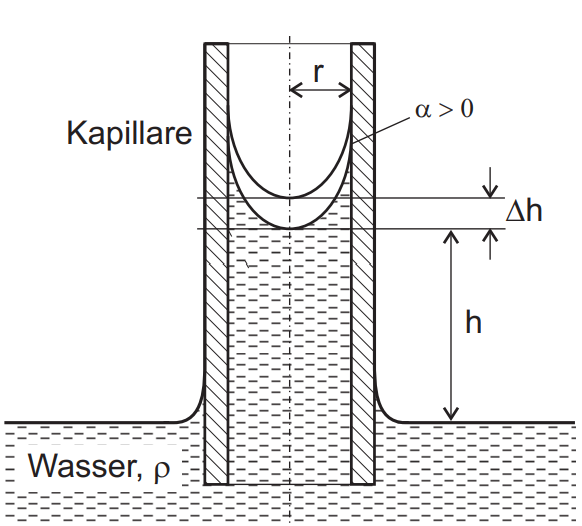
\includegraphics[width=\linewidth]{pics/Kapillare.png}
            \caption[Messung nach der Kapillarmethode]{Zur Messung nach der Kapillarmethode. $r$ Radius der Kapillare, $h$ Steighöhe, $\rho$ Dichte der Flüssigkeit. Für vollständig benetzende Flüssigkeiten ist der Randwinkel $\alpha = 0$.}
            \label{fig:Kapillare}
        \end{minipage}
    \end{center}
 \end{figure}


% \begin{figure}[htbp] %Todo add graphic
%     \centering
%     \caption[Versuchsanordnung]{Bla Bla}
%     \label{fig:Versuchsanordnung}  % after caption for right numbering
    
%     \includegraphics[width=0.35\textwidth]{NAME.png}
% \end{figure}

\section{Geräteliste}
\label{sec:geraeteliste}
\begin{center}
    \captionof{table}[Geräteliste]{Verwendete Geräte}  % optionales Argument wird in Verzeichnissen verwendet, essentielles Argument direkt im Text
    \label{tab:geraeteliste}
    \vspace{3mm}  % vertical space 3 mm
    \begin{tabular}{|c|c|c|c|}
        \hline
        Gerät                    & Hersteller & Gerätenummer & Unsicherheit       \\ \hline
        Kathetometer             & -          & axx          & 0,5 Skalenabstände \\ \hline
        Kamera                   & -          & bxx          & -                  \\ \hline
        Federwaage               & -          & cxx          & \SI{1}{\mN}        \\ \hline
        Lenardbügel              & -          & dxx          & -                  \\ \hline
        Ring                     & -          & fxx          & -                  \\ \hline
        Kapillaren               & -          & gxx          & -                  \\ \hline
        Mikrometer               & -          & hxx          & \SI{10}{\um}       \\ \hline
        Schublehre               & -          & ixx          & \SI{0.05}{\mm}     \\ \hline
        Stativ des Kathetometers & -          & jxx          & \SI{0.1}{\mm}      \\ \hline
        \hline
    \end{tabular}
\end{center}


\section{Versuchsdurchführung und Messergebnisse}
\label{sec:versuchsdurchfuehrung_messergebnisse}
Es wurde die Oberflächenspannung von den verschiedenen Flüssigkeiten 
auch auf verschiedene Arten festgestellt da bietet es sich an diese
auch seperat durchzugehen.

\subsection{Oberflächenspannung nach Lenard}
Wie in \nameref{sec:voraussetzungen_grundlagen} schon erwähnt wurde ist hier
Methode von Lenard angewendet.
\subsubsection{Ablauf}
\begin{enumerate}
    \item Ein Behälter wird mit der zu untersuchenden Flüssigkeit befüllt,
        bis der Flüssigkeitsstand so hoch ist, dass das ganze Objekt bedeckt
        werden kann.
    \item Der Behälter wird auf eine höhenverstellbare Unterlage plaziert.
    \item Das Objekt wird nun an der Federwaage befestigt. Diese wird danach so 
        eingestellt, dass sie auf Null justiert ist, wenn das Objekt 
        in die Flüssigkeit eintaucht und von dieser benetzt wird.
    \item Nun wird Behälter langsam hinuntergelassen, bis der Flüssigkeitsfilm
        reißt und man die maximale Kraft von der Federwaage durch
        die Kameraaufzeichnung ablesen kann.
    \item Das Bild mit dem Messwert wird dann mittels dem Bildbearbeitungsprogramm
        GIMP untersucht. Die maximale Anzahl an sichtbaren Skalenstrichen 
        wurden als Maßstab verwendet um $\pm 7$ px Ableseauflösung zu
        haben.
\end{enumerate}
Diese Methode wurde für alle Messwerte wiederholt, sowohl für die Wasser
als auch für die Seifenlauge Messung und auch für jedes Objekt. Mit dieser 
Methodik sind folgende Messwerte zustandegekommen.


\subsubsection{Messung Seifenlauge}
\begin{center}
\captionof{table}{Messreihen der maximalen Kraft in der Seifenlauge links mit Bügel ($F_{Bügel}$) rechts mit Ring ($F_{Ring}$). Wobei $\mu$ der Mittelwert und $\hat \sigma$ die Standardabweichung des Mittelwerts der Messswerte sind.}
    \label{tab:seifenwerte}
\begin{tabular}{cc}%
\begin{tabular}[t]{l|S}
    i  & $F_{Bügel}$\, / \,mN     \\ \hline
	1  & \num{7.7(4)} \\
	2  & \num{7.6(4)} \\
	3  & \num{7.9(4)} \\
    4  & \num{8.5(4)} \\
    5  & \num{8.3(4)} \\
    $\mu \pm \hat \sigma$ & \num{8.0(2)}\\ \hline
\end{tabular}
\quad
\begin{tabular}[t]{l|S}
    i  & $F_{Ring}$\, / \,mN     \\ \hline
    1  & \num{15.3(4)} \\
    2  & \num{15.7(4)} \\
	3  & \num{16.0(4)} \\
	4  & \num{16.3(4)} \\
	5  & \num{15.6(4)} \\
    $\mu \pm \hat \sigma$ & \num{15.8(2)}\\ \hline
\end{tabular}
\end{tabular}
\end{center}

\subsubsection{Messung Wasser}

\begin{center}
    \captionof{table}{Messreihen der maximalen Kraft im Wasser links mit Bügel ($F_{Bügel}$) rechts mit Ring ($F_{Ring}$). Wobei $\mu$ der Mittelwert und $\hat \sigma$ die Standardabweichung des Mittelwerts der Messwerte sind.}
    \label{tab:wasserwerte}
\begin{tabular}{cc}%
\begin{tabular}[t]{l|S}
    i  & $F_{Bügel}$\, / \,mN     \\ \hline
	1  & \num{14.6(3)} \\
	2  & \num{14.5(3)} \\
	3  & \num{15.2(3)} \\
    4  & \num{15.0(3)} \\
    5  & \num{15.5(3)} \\
    $\mu \pm \hat \sigma$ & \num{15.0(2)}\\ \hline
\end{tabular}
\quad
\begin{tabular}[t]{l|S}
    i  & $F_{Ring}$\, / \,mN     \\ \hline
    1  & \num{26.1(3)} \\
    2  & \num{25.9(3)} \\
	3  & \num{26.1(3)} \\
	4  & \num{24.6(3)} \\
	5  & \num{25.1(3)} \\
    $\mu \pm \hat \sigma$ & \num{25.6(3)}\\ \hline
\end{tabular}
\end{tabular}
\end{center}

Weiters wurde auch die innere Bügellänge und der
Außendurchmesser des Ringes, durch das Messen mit einer Schublehre, bestimmt.

\begin{table}[h]
    \centering
    \caption{Zusätzliche Messungen der inneren Bügellänge und des Außendurchmessers des Ringes}
    \label{tab:längen}
    \begin{tabular}{S|S}
        $L_{Bügel}$ & $\varnothing_{Ring}$ \\
        \SI{10.035(5)}{\cm} & \SI{6.000(5)}{\cm} \\
    \end{tabular}
\end{table}

\subsection{Kapillaren}
Da nicht nur eine Methode verwendet wurde um die Oberflächenspannung von Wasser
zu bestimmmen, wird in dieser Subsektion die Durchführung dieser Methode
erläutert und die daraus resultierenden Ergebnisse angeführt.

\subsubsection{Ablauf}
\begin{enumerate}
    \item Eine Kapillare wird mit dem Mikrometer abgemessen um, den Außendurchmesser
        der Kapillare zu bestimmen.
    \item Die Kapillare wird so plaziert, dass im Kathetometer die Wände
        der Kapillare gut sichtbar sind und mittels der Skala (oder dem
        Bildbearbeitungsprogramm) das Verhältnis des Außendurchmessers und
        des Innendurchmessers ablesbar ist.
    \item Da der Durchmesser der Kapillare bekannt ist, ist es möglich den
        Innendurchmesser dieser Kapillare zu bestimmen.
    \item Nun wird die Kapillare vertikal in ein Behälter mit Wasser plaziert,
        sodass der Kapillareffekt stattfinden kann.
    \item Damit nun die, durch den Kapillareffekt enstandene, Höhenänderung
        in der Kapillare gemessen werden kann wird das Kathetometer verwendet.
        Da dies ein höhenverstellbares Stativ mit einer Millimeterskala besitzt.
    \item Das Kathetometer so eingestellt wird, dass der Wasserspiegel
        bei zb. Skalenstrich 30 ist. Als Referenz kann nun, der bei dieser 
        Einstellung erhaltene, Höhenwert verwendet werden.
    \item Nun stellt man das Kathetometer so ein, dass der Meniskus beim
        gleichen Skalenstrich wie oben ist. Die Differenz zwischen Refenenzwert 
        und diesem Messwert ist die Höhenänderung, aufgrund des Kapillareffekts.
\end{enumerate}

Diese Prozedur wird für alle drei Kapillaren wiederholt.
Da die Unsicherheit in der Messung des Außendurchmessers $\pm$ 0,01 mm
der Kapillaren natürlich
beeinflusst, sowie auch das Ablesen mittels dem Bildbearbeitungsprogramm $\pm$ 15px 
(größer da der Übergang schlechter zusehen war). Komibniert man diese Fehler bekommt
man einen Fehler von ca. $\pm$ 0,025 mm.
Die Werte der Messungen sind in den folgenden Tabellen angeführt: 


\begin{table}[h]
    \centering
    \caption{Zusätzliche Messungen der inneren Bügellänge und des Außendurchmessers des Ringes}
    \label{tab:kappidata}
    \begin{tabular}{c|S|S|S}
        Kapillare Nr.                             & \num{1}                  & \num{2}                   & \num{3}                  \\ \hline
        Außendurchmesser / mm                     & \num{1.775(5)}           & \num{1.549(5)}            & \num{1.560(5)}           \\
        Verhältnis Innen zu Außen / \si{\px\per\px} & \num{927(15) / 1307(15)} & \num{1377(15) / 1900(15)} & \num{770(15) / 1048(15)} \\
        Innerer Radius ($r_i$) / mm               & \num{0.63(3)}           & \num{0.56(3)}             & \num{0.57(3)}            \\
        Referenzhöhe / cm                         & \num{4.66(1)}            & \num{4.66(1)}             & \num{4.66(1)}            \\
        $\Delta h$ / cm                           & \num{0.64(2)}            & \num{0.96(2)}             & \num{0.64(2)}            \\
    \end{tabular}
\end{table}




% \begin{center}
%     \captionof{table}[MESSUNG]{Bla Bla}%Ausfüllen
%     \label{tab:messergebnisse}
%     \vspace{3mm}
%     \begin{tabular}{|cc|cc|cc|}
%         \hline
%         n   & $10 \cdot T$  & n  & $10 \cdot T$ & n  & $10 \cdot T$ \\ \hline
%         1   & 29,12         & 11 & 29,11        & 21 & 29,06        \\ \hline
%         2   & 29,06         & 12 & 29,03        & 22 & 29,09        \\ \hline
%         3   & 29,16         & 13 & 29,06        & 23 & 29,06        \\ \hline
%         4   & 29,04         & 14 & 29,13        & 24 & 29,11        \\ \hline
%         5   & 29,04         & 15 & 29,03        & 25 & 29,08        \\ \hline
%         6   & 29,19         & 16 & 29,07        & 26 & 29,04        \\ \hline
%         7   & 29,13         & 17 & 29,06        & 27 & 29,04        \\ \hline
%         8   & 29,03         & 18 & 29,08        & 28 & 29,04        \\ \hline
%         9   & 29,10         & 19 & 29,06        & 29 & 29,03        \\ \hline
%         10  & 29,08         & 20 & 29,00        & 30 & 29,03        \\ \hline
%         \hline
%     \end{tabular}
% \end{center}
\section{Auswertung}
\label{sec:auswertung}

Die Auswertungen der unterschiedlichen Methoden sind in zwei Unterkapitel
gegliedert.

\subsection{Methode nach Lenard}
Kombiniert man die Messwerte der Tabellen (\ref{tab:seifenwerte},\ref{tab:wasserwerte},\ref{tab:längen}) mit der 
\autoref{eq:Oberflaechenspannung_spezial} erhaltenen wir folgende Werte für 
die Oberflächenspannung $\sigma$:

\begin{table}[h]
    \centering
    \caption{Ergebnisse für die Oberflächenspannungen $\sigma$ von Wasser und Seifenlauge, welche durch die Methode von Lenard ermittelt worden sind}
    \label{tab:results_lenard}
    \begin{tabular}{c|S}
        Oberflächenspannung von: & $\sigma / \frac{\text{mN}}{\text{m}}$ \\ \hline
        Wasser mittels Bügel & \num{74.5(10)} \\
        Wasser mittels Ring & \num{68(2)} \\
        Seifenlauge mittels Bügel & \num{39.9(10)} \\
        Seifenlauge mittels Ring & \num{41.8(10)} \\
    \end{tabular}
\end{table}

Für die Unsicherheitfortpflanzung ist wie zuvor erwähnt die verallgemeinerte
Gaußmethode verwendet worden und ist mittels Python \verb|scipy| ausgewertet
worden.
\subsection{Kapillareffekt}
Um die Oberflächenspannung zu bestimmen mittels dem Kapillareffekt werden die
Daten der \autoref{tab:kappidata} und die \autoref{eq:Oberflauechenspannung_Kapillare}
verwendet. Wie auch im vorigen Teil sind die Unsicherheitintervalle mittels
Python errechnet worden. Wobei $\rho=$ \SI{0.998207}{\gram\per\ml} die 
Dichte des Wasser von der Website \cite{Wagner2002} für \SI{20}{\celsius} 
entnommen worden ist. 

\begin{table}[h]
    \centering
    \caption{Ergebnisse für die Oberflächenspannungen $\sigma$ von Wasser unterverwendung des Kapillareffekts}
    \label{tab:results_kappi}
    \begin{tabular}{c|S|S|S}
        Kapillare & 1 & 2 & 3 \\ \hline
        $\sigma / \frac{\text{mN}}{\text{m}}$ & \num{19(2)} &\num{26(1)} & \num{18(1)} \\
    \end{tabular}
\end{table}

\section{Diskussion und Zusammenfassung}
\label{sec:diskussion_zusammenfassung}
% %Aufzählung was scheiße glaufen is

Wie in \autoref{tab:endwerte} ersichtlich weichen die Werte der verschiedenen
Methoden deutlich von einander ab.
Gründe für die unterschiedlichen Werte für die Oberflächenspannung von Wasser
der zwei Methoden sind zb.:
\begin{itemize}
    \item Messungenauigkeiten des Radien, der Dichte, der 
        Erdbeschleunigung und der Höhendifferenz bei der Methode des
        Kapillareffekts
    \item Messungenauigkeiten der maximalen Abrisskraft und der Länge der
        mit dem Wasser im Kontakt stehenden Fläche bei der Methode nach 
        Lenard
    \item Die Methode des Kapillareffekts hat viel mehr Variabeln wodurch
        die Unsicherheitsintervalle drastisch größer werden als bei der
        Methode nach Lenard
\end{itemize}

Bei der Kapillareffekt Methode würde man viel mehr Geräte benötigen, welche
zudem auch sehr genau Messungen vollziehen müssten, da jede Variabel einen
enormen Fehlerverursachen könnte. Aufgrund der Einfachheit und der geringen
Anzahl der zumessenden Variabeln ist die Methode nach Lenard zu bevorzugen.
Dies reflektiert auch der Vergleich mit dem Literaturwert, welcher \SI{72.75}{\mN\per\meter}
\cite{2021Oberflache}
bei \SI{20}{\celsius}. 

Da die genaue Zusammensetzung der Seifenlauge nicht bekannt ist, macht es
keinen Sinn den gemessen Wert mit einem genauen Literaturwert zu vergleichen.
Es macht nur Sinn den gemessen Wert größenordnungsmäßig mit dem Literaturwert 
zu vegleichen und zu schauen ob dieser auch niedriger als der vom Wasser ist.
Laut Literatur liegt der Wert bei \SI{30}{\mN\per\meter} \cite{Roth2016}, was größenordnungsmäßig
dem gemessen Wert entspricht  und auch ungefähr die Hälfte von der Oberflächenspannung
von Wasser beträgt.



\begin{table}[h]
\centering
\caption{Tabelle der Resultate für die Oberflächenspannungen der verschiedenen Flüssigkeiten}
\label{tab:endwerte}
\begin{tabular}{c|S|S}
    Typ         & {Wasser}              & {Seifenlauge}         \\ \hline
    Lenardbügel & \SI{74.5(10)}{\mN\per\meter} & \SI{39.9(10)}{\mN\per\meter} \\
    Ring        & \SI{68(2)}{\mN\per\meter} & \SI{41.8(10)}{\mN\per\meter} \\
    Kapillare 1 & \SI{19(2)}{\mN\per\meter}   & {-}                          \\
    Kapillare 2 & \SI{26(1)}{\mN\per\meter}   & {-}                          \\
    Kapillare 3 & \SI{18(1)}{\mN\per\meter}   & {-}
\end{tabular}
\end{table}


Alle Werte passen größenordnungsmäßig mit den Literaturwerten überein. Würde
man genauere Werte benötigen sollte man eher die Methode von Lenard verwenden
und genauere Messungen vollziehen.

% Literaturtabelle
\newpage
%\bibliographystyle{unsrt}
\printbibliography
%\bibliography{oberflaeche} %Todo .bib befüllen zb.: mit JabRef (Empfehlung der Redaktion)

\listoffigures

\listoftables

\end{document}
